\documentclass{article}
\usepackage{amsmath}
\usepackage{tcolorbox}
\usepackage[margin=0.5in]{geometry} 
\usepackage{amsmath,amsthm,amssymb,amsfonts, fancyhdr, color, comment, graphicx, environ}
\usepackage{float}
\usepackage{xcolor}
\usepackage{mdframed}
\usepackage[shortlabels]{enumitem}
\usepackage{indentfirst}
\usepackage{mathrsfs}
\usepackage{hyperref}
\usepackage{extarrows}
\graphicspath{./}
\makeatletter
\newcommand*{\rom}[1]{\expandafter\@slowromancap\romannumeral #1@}
\makeatother

% Define a new environment for problems
\newcounter{problemCounter}
\newtcolorbox{problem}[2][]{colback=white, colframe=black, boxrule=0.5mm, arc=4mm, auto outer arc, title={\ifstrempty{#1}{Problem \stepcounter{problemCounter}\theproblemCounter}{#1}}}

% \renewcommand{\labelenumi}{\alph{enumi})}
\def\zz{{\mathbb Z}}
\def\rr{{\mathbb R}}
\def\qq{{\mathbb Q}}
\def\cc{{\mathbb C}}
\def\nn{{\mathbb N}}
\def\ss{{\mathbb S}}

\newtheorem{theorem}{Theorem}[section]
\newtheorem{corollary}{Corollary}[theorem]
\newtheorem{lemma}[theorem]{Lemma}
\newtcolorbox{proposition}[1][]{colback=white, colframe=blue, boxrule=0.5mm, arc=4mm, auto outer arc, title={Proposition #1}}
\newtcolorbox{definition}[1][]{colback=white, colframe=violet, boxrule=0.5mm, arc=4mm, auto outer arc, title={Definition #1}}
\newcommand{\Zmod}[1]{\zz/#1\zz}
\newcommand{\partFrac}[2]{\frac{\partial #1}{\partial #2}}

\newcommand\Mydiv[2]{%
$\strut#1$\kern.25em\smash{\raise.3ex\hbox{$\big)$}}$\mkern-8mu
        \overline{\enspace\strut#2}$}

\begin{document}

\begin{center}
    Math 741
    \hfill Homework 2
    \hfill \textit{Stephen Cornelius}
\end{center}

\begin{problem} \\ 
\begin{enumerate}[a)]
    \item Write a program that can evaluate the numbers $c_{n,k}$ in Pascal's triangle using a recurrence relation.
Define $c_{n,0} = 1$ for all $n \geq 0$ and $c_{0,k}=0$ for $k \geq 0$. Then the entries for $n + 1$ and be computed from the entries for $n$ using 
\[
		c_{n+1,k} = c_{n,k} + c_{n,k-1}.
	\]
	Print a table of entries in Pascal's triangle for $0 \leq n \leq 7$ and $0 \leq k \leq 7$. You should find that $c_{n,k} = 0$ for $k > n$, and those terms can be left blank in your table.


	\item Extend your program so that it prints ASCII art, displaying a "." character for each even number and a "\#" character for each odd number. Hence the first few lines would be
	\begin{verbatim}
        #
        ##
        #.#
        ####
    \end{verbatim}
	Using your program, extend this output to $n = 31$.
\end{enumerate}
\end{problem}
\begin{enumerate}[a)]
    \item Originally, I implemented the recurrence relation in a function (\verb|PascalTriangle_Coefficients(int n, int k)|) that called itself. I then called this function in \verb|main()|. While this worked, I realized that it was calculating the same values over and over again which made it very slow. Instead wrote a function (\verb|Generate_Pascal_Triangle(int numRows)|) that output a vector of vectors that stored the values as they were calculated. This made it much faster. I also added a function to print the triangle in a nice format. Below is the output of the program when I input 7 rows. \\ 
    \begin{center}
        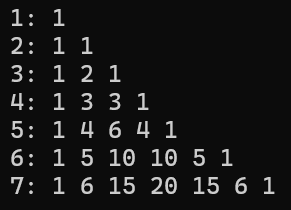
\includegraphics[width=0.5\textwidth]{OpHw1_1a.png}
    \end{center}
    \newpage
    \item I was tasked with outputting a table of for Pascal's triangle where each even number was replaced by a "." and each odd number was replaced by a "\#". I modified my previous program to do this. Below is the output of the program when I input 31 rows. \\
    \begin{center}
        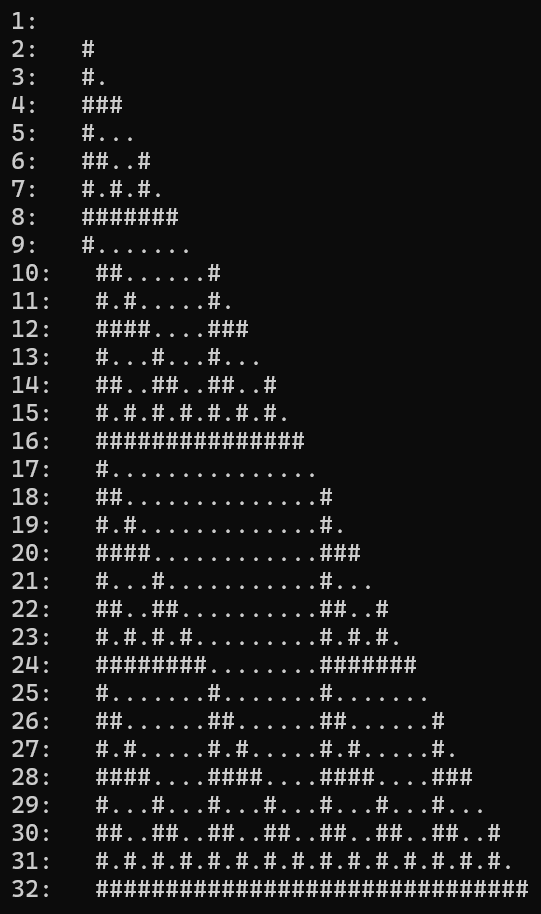
\includegraphics[width=0.5\textwidth]{OpHw1_1b.png}
    \end{center}
\end{enumerate}


\begin{problem} \\ 
    \begin{enumerate}[a)]
        \item Write a function that takes in two arrays and preforms matrix multiplication. \\
    Your function's signature should be:
    \begin{verbatim}
        void mat_mul(const double* A, const double* B, double* C, int m, int n, int p);
    \end{verbatim}
    The function should compute $C = AB$, where $A \in \rr^{m\times n}, B \in \rr^{n \times p}$, and $C \in \rr^{m \times p}$. Test your program on the matrices
    \[
        A = \begin{pmatrix}
            0 & 1 & 2 \\
            0 & 1 & 2 
        \end{pmatrix},
        \quad 
        B = \begin{pmatrix}
            0 & 1 & 2 & 3 \\
            0 & 1 & 2 & 3 \\
            0 & 1 & 2 & 3 
        \end{pmatrix},
    \]
    which can be generated using the provided \verb|gradient_matrix| function.
    \item \textbf{Optional.} Measure the time $T(m)$ to generate two random matrices $A, B \in \rr^{m\times m}$ and multiply them together using your routine. Calculate $T(m)$ for $m = 100, 200, 300, \dots , 1600$. Use linear regression on fit the data to 
    \[
        T(m) = Cm^\alpha
    \] 
    for constants $C$ and $\alpha$, comment on whether the value $\alpha$ is consistent with your matrix multiplication algorithm.
    \end{enumerate}
    
    
\end{problem}




\end{document}